\section{\texttt{gzip} Compression Details}
\label{app:sec:gzip_compression_details}

\texttt{gzip} is a lossless data compression algorithm that combines two primary techniques: LZ77 compression and Huffman coding. Here, we provide additional technical details on how \texttt{gzip} works.

\paragraph{LZ77 Compression:}
LZ77 works by identifying repeated substrings in the input text and replacing them with backward references. Mathematically, LZ77 can be described as follows:

Given an input sequence \( S = s_1, s_2, \dots, s_n \), the algorithm searches for the longest prefix of the remaining sequence \( S' = s_i, s_{i+1}, \dots, s_n \) that matches a substring within a predefined window of previous characters. If a match is found, it is replaced by a tuple \( (d, l, c) \), where:
\begin{itemize}
    \item \( d \) is the distance from the current position to the start of the matching substring,
    \item \( l \) is the length of the matching substring, and
    \item \( c \) is the character following the match (if any).
\end{itemize}
For example, the substring \( s_i, s_{i+1}, \dots, s_{i+l-1} \) can be replaced by the tuple \( (d, l, c) \), thereby reducing redundancy in the data.

\paragraph{Huffman Coding:}
After applying LZ77, \texttt{gzip} employs Huffman coding to further reduce the size of the compressed data. Huffman coding assigns variable-length codes to symbols based on their frequency of occurrence, with shorter codes assigned to more frequent symbols.

The expected length \( L(X) \) of the Huffman code for a sequence of symbols \( X = x_1, x_2, \dots, x_n \) is calculated as:
\[
L(X) = \sum_{i=1}^{n} p(x_i) \cdot \text{len}(C(x_i)),
\]
where:
\begin{itemize}
    \item \( p(x_i) \) is the probability of symbol \( x_i \),
    \item \( \text{len}(C(x_i)) \) is the length of the Huffman code for \( x_i \).
\end{itemize}
This further minimizes the size of the compressed data by leveraging the statistical properties of the input.

\paragraph{Combined \texttt{gzip} Compression:}
The total compressed size \( C(S) \) after applying both LZ77 and Huffman coding can be approximated as the sum of the lengths of the backward references and the Huffman-coded symbols:
\[
C(S) = \sum_{(d, l, c)} \text{len}(d, l, c) + \sum_{i=1}^{n} \text{len}(C(x_i)).
\]

\paragraph{Normalized Compression Distance (NCD):}
\texttt{gzip}’s effectiveness in data selection stems from its ability to measure the alignment between two sequences \( A \) and \( B \) based on how efficiently they compress together. The \textbf{Normalized Compression Distance (NCD)} is given by:
\[
NCD(A, B) = \frac{C(A \oplus B) - \min(C(A), C(B))}{\max(C(A), C(B))},
\]
where \( C(A) \) and \( C(B) \) are the compressed lengths of sequences \( A \) and \( B \), and \( C(A \oplus B) \) is the length of the compressed concatenation of both sequences. 
A lower NCD indicates greater alignment between the sequences.

% If the two objects are very similar, their combined compressed size should approach the size of the simpler one, because you are just adding redundant information.

\subsection{Why Use Compression?}

Compression algorithms, such as \texttt{gzip}, provide a computationally efficient way to detect patterns and minimize redundancy in data. 
\paragraph{Limitations of n-grams:} Many traditional methods, including hashed n-grams, focus on capturing immediate textual correlations by simplifying text into discrete, fixed-size buckets. 
Although these techniques are computationally efficient, they may not adequately capture syntactic or structural relationships within the data. Additionally, the introduce noise due to collisions during hashing.

\paragraph{Challenges with Neural Embeddings:} Neural embeddings offer a powerful tool for capturing semantic relationships, but they come with significant computational costs. These embeddings are typically pre-trained on large corpora and fine-tuned for specific tasks, which requires substantial resources. Given the scalability challenges of embedding-based methods, we conjecture that a simpler method like compression can provide a more scalable and resource-efficient alternative.

We hypothesize that compression -- in this case \texttt{gzip}, but perhaps a different compression algorithm --serves as a strong proxy for capturing syntactic and structural relationships in textual sequences. 
\texttt{gzip}’s ability to compress data based on redundancy minimization can be leveraged as a metric to align text with a target distribution. 


\subsection{Composition of the Source Dataset for AutoFormalization}
\label{app:subsec:dataset_composition_af}
The source dataset for the AutoFormalization task was compiled from a variety of datasets to ensure a diverse mix of mathematical, general textual, and code-related content. Below are the details of the datasets included:

\begin{itemize}
    \item \textbf{UDACA/AF:} 4,300 samples from informal formalization statements.
    \item \textbf{C4:} 10,000 samples from the clean crawl of the internet, ensuring a broad linguistic variety.
    \item \textbf{LeanDojo:} 10,000 samples from task-oriented proofs and tactics.
    \item \textbf{LeanDojo Informalized:} 10,000 samples combining traced tactics with informal descriptions, aiming to bridge formal reasoning and natural language.
    \item \textbf{UDACA/AF-split:} 10,000 samples, a variant of the UDACA/AF dataset with split annotations.
    \item \textbf{WikiText:} 10,000 samples from a collection of professionally curated articles, providing a rich linguistic framework.
    \item \textbf{Algebraic Stack:} Samples from various subsets of mathematical and programming languages, capped at 10,000 samples per subset or fewer if the total subset size was under this threshold.
\end{itemize}

Each dataset was selected to complement the others by covering different aspects of language use, from technical to informal, ensuring the model's exposure to a wide range of linguistic structures and contents. The total dataset size aggregated to approximately 185,000 sequences, which were then subjected to alignment scoring and further processing for model training.

\subsection{Composition of the Source Dataset for Code Generation}
\label{app:subsec:dataset_composition_code}

The source dataset for the Code Generation task was assembled from various data sources to provide a diverse range of coding and natural language contexts. Below are the details of the datasets included:

\begin{itemize}
    \item \textbf{MBPP (Google Research):} A total of 964 samples focusing on Python coding challenges.
    \item \textbf{Python Code Instructions (18k Alpaca):} 5,000 sequences providing natural language prompts for Python code, fostering a practical approach to code generation.
    \item \textbf{Python Docstrings (Calum/The Stack):} 5,000 sequences each of Python function docstrings integrating detailed natural language documentation of python functions.
    \item \textbf{Python Docstrings (Calum/The Stack):} 5,000 sequences each of Python function code bodies, integrating raw python code without documentation.
    \item \textbf{C4 (AllenAI):} 10,000 samples from a clean web crawl.
    \item \textbf{WikiText:} 10,000 samples from a collection of curated articles, providing rich natural language training material.
    \item \textbf{Algebraic Stack:} A selection of sequences from various programming language subsets, each capped at 10,000 samples or the total subset size if less than this threshold.
\end{itemize}

This combination of datasets was specifically chosen to challenge our methods 's ability to choose syntactically correct and functionally accurate Python code, while also responding appropriately to natural language prompts. 

\subsection{Hyperparameters for Model Fine-Tuning}

All models in our experiments were fine-tuned with the following unified setup, aimed at ensuring a consistent evaluation across different models and data selection strategies.

\paragraph{Models and Tokenizer:}
The fine-tuning was performed using the following models:
\begin{itemize}
    \item InterLM-Math-Plus-1.8B
    \item Gemma2-2B
    \item Mistral7B
\end{itemize}

\paragraph{Training Settings:}
The key hyperparameters used across all models are as follows:
\begin{itemize}
    \item \textbf{Block Size:} 1024 tokens
    \item \textbf{Learning Rate:} $7.5 \times 10^{-7}$
    \item \textbf{Batch Size:} 4 (per device)
    \item \textbf{Number of Epochs:} 1
    \item \textbf{Weight Decay:} 0.01
    \item \textbf{Maximum Gradient Norm:} 1.0
\end{itemize}

Training was facilitated using the \texttt{Trainer} class from Hugging Face's Transformers library, with the Accelerate library handling model parallelism to efficiently utilize available computational resources.

\paragraph{Evaluation Metrics:}
For model evaluation, we employed:
\begin{itemize}
    \item \textbf{Cross-Entropy Loss} at the end of training to measure the effectiveness of the fine-tuning.
\end{itemize}

Fine-tuning was performed under controlled conditions to ensure fair comparison between data selected by \texttt{ZIP-FIT}, DSIR, and manual curation methods. The effectiveness of each method was assessed based on how the models performed on the ProofNet and HumanEval.

\paragraph{Data Handling and Logging:}
All logs, model checkpoints, and tokenizer settings were systematically saved in designated directories for thorough analysis post-experiment

This comprehensive and standardized approach to fine-tuning ensures that our experimental results are robust, reproducible, and transparent, providing clear insights into the effectiveness of the data selection methodologies employed in our study.

\section{Rationale for the Method Name \texttt{ZIP-FIT}}

We chose the name \textbf{ZIP-FIT} for two reasons:
\begin{enumerate}
    \item \textbf{ZIP} refers to the use of \texttt{gzip} compression for data selection, where compression aligns the data for better future fine-tuning (or \textbf{FITting}).
    \item The name also references scaling laws, as \texttt{ZIP-FIT} consistently reduces loss faster than competing methods, implying better power-law scaling parameters, drawing a parallel to \textbf{Zipf's law} \cite{piantadosi2014zipf}, which describes similar scaling behavior in language models.
\end{enumerate}

\textit{Remark:} Zipf's law \cite{piantadosi2014zipf} describes the inverse relationship (thus power law $f(r) \propto 1/r^s$, where $r$ is the rank and $f(r)$ is the frequency of the word with rank $r$) between a word's frequency and its rank in natural language, a pattern that reflects scaling behavior. 
Rank in this context is the position of the word after sorting with respect to frequency in the text.

\newpage

\section{Additional Experimental Results: data selection for efficient fine-tuning using \texttt{ZIP-FIT}}
\label{sec:more-af-plots}
\begin{figure*}[!ht]
    \centering
    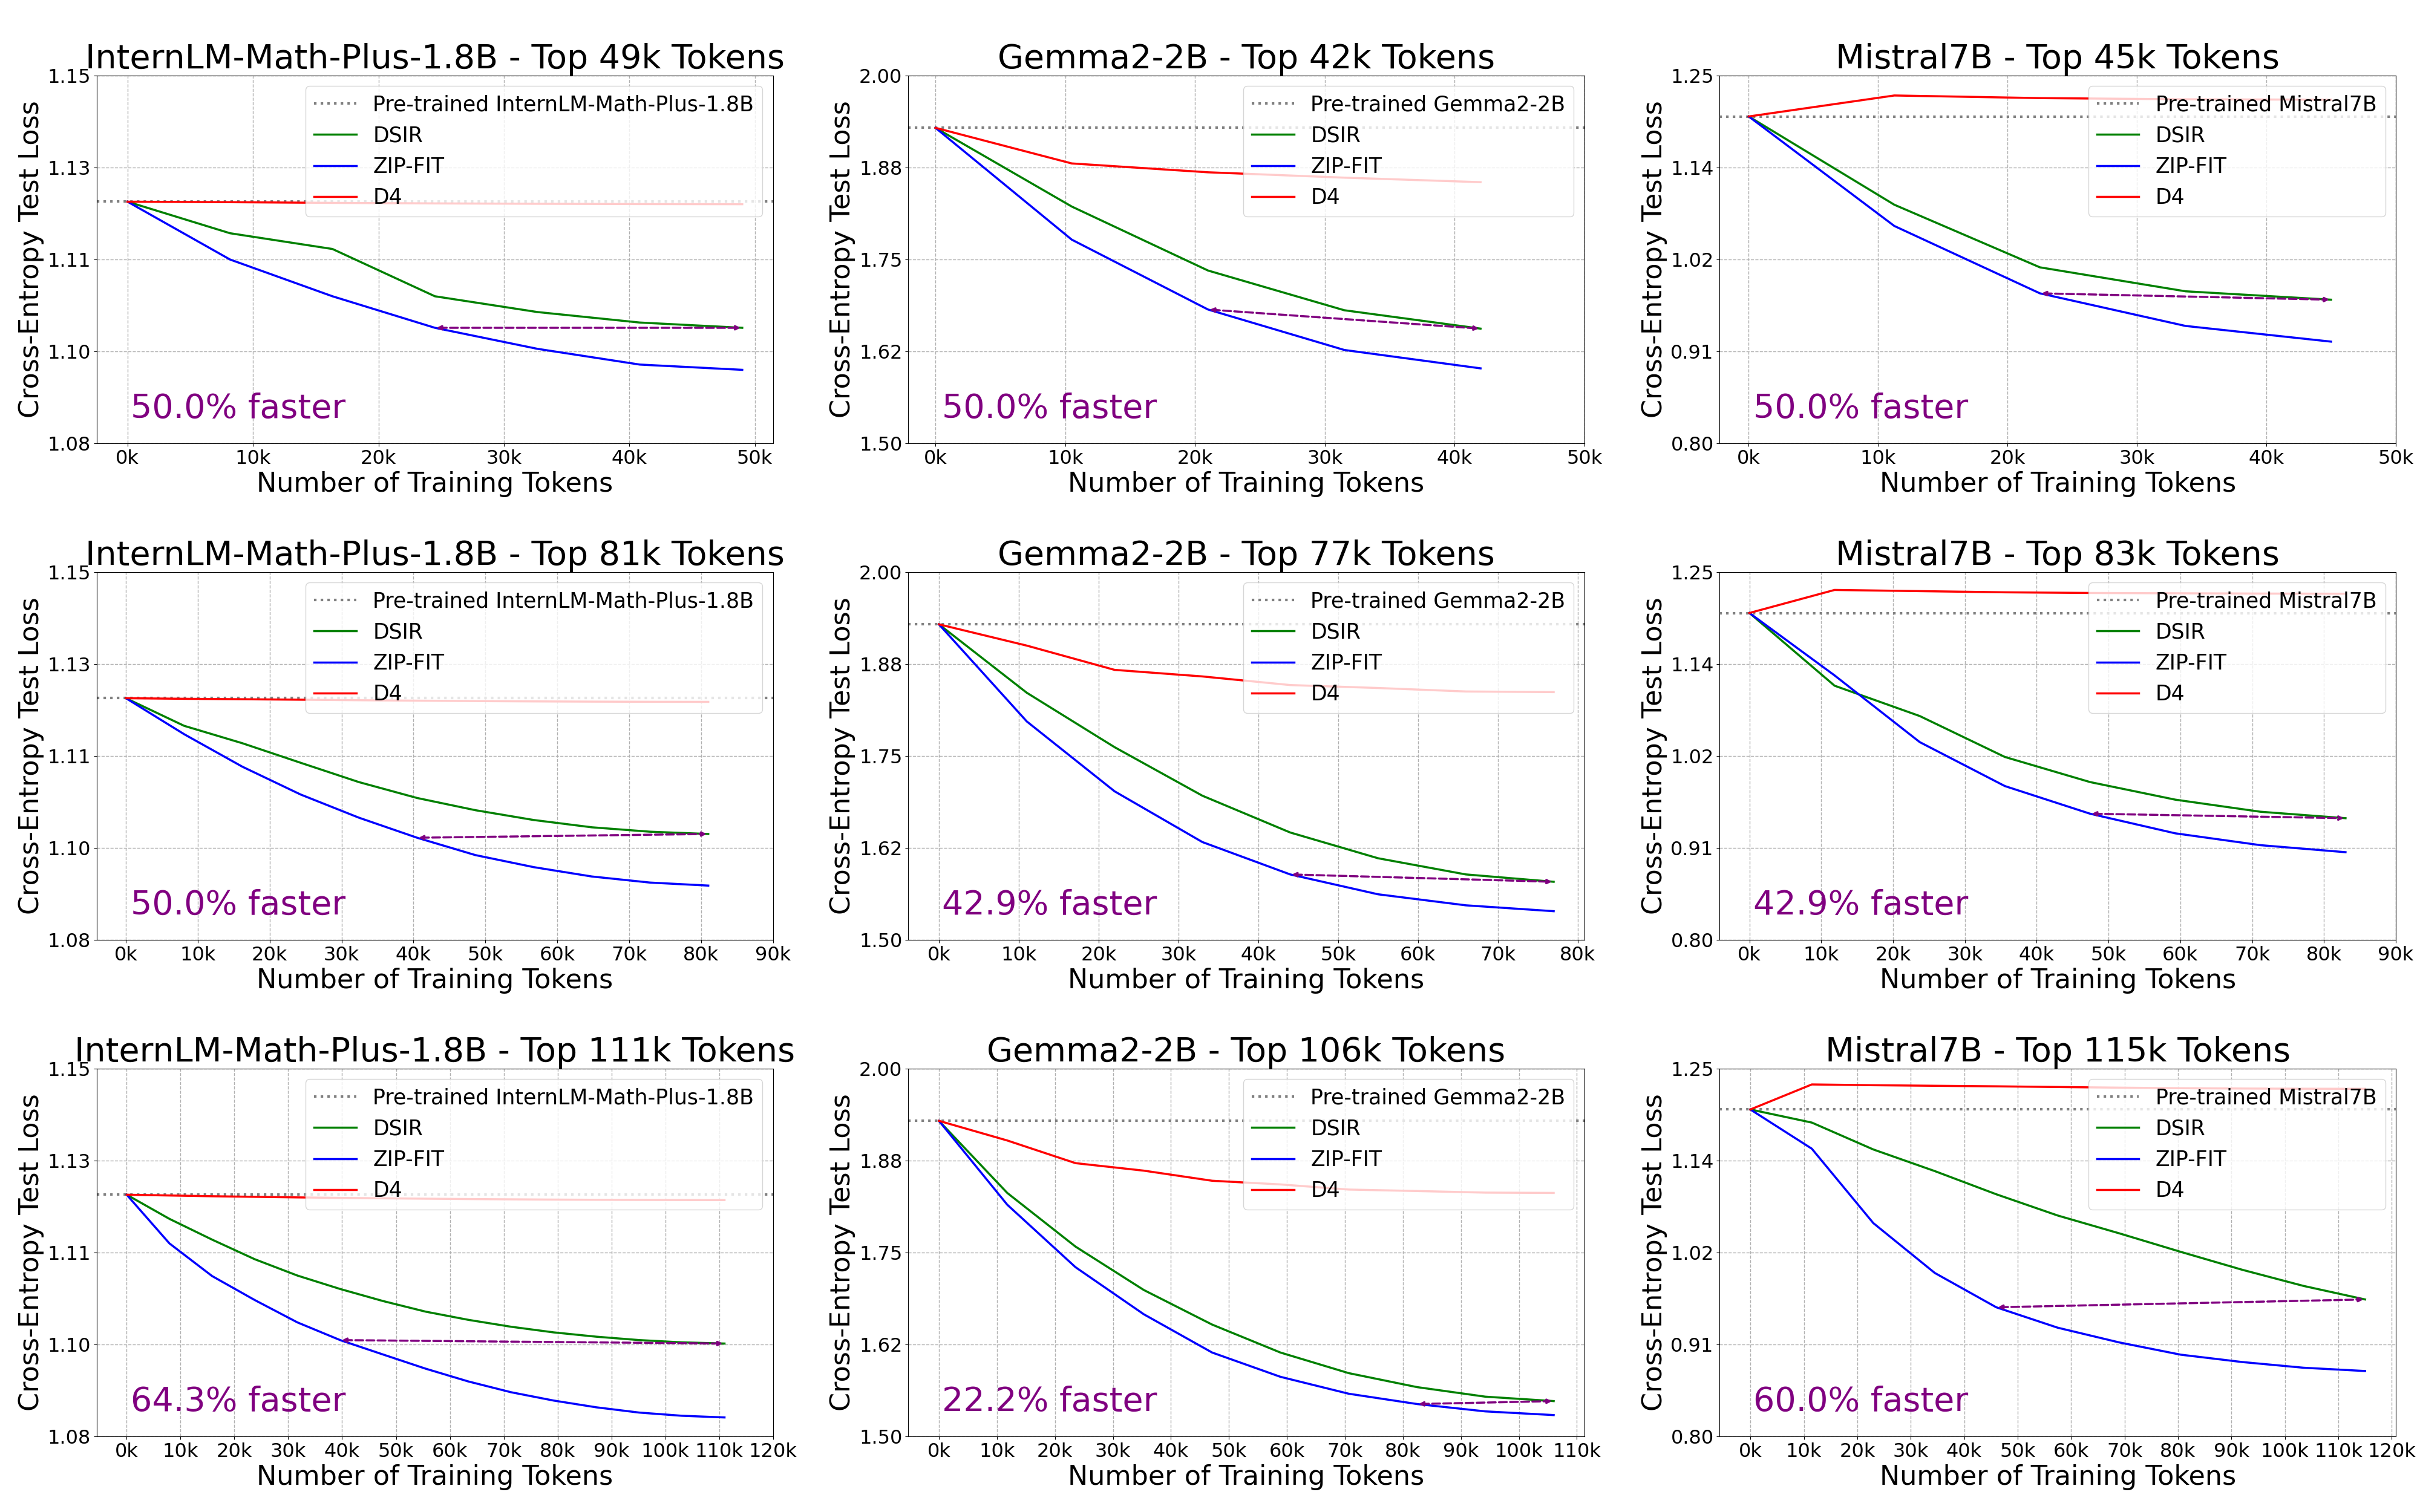
\includegraphics[width=\textwidth]{plots/af_remaining_plot.png}
    \caption{\textbf{\texttt{ZIP-FIT} consistently achieves a lower test loss at a faster rate compared to D4 and DSIR for Autoformalization}. The plots show the cross-entropy test loss against the number of training tokens for three models (InterLM-Math-Plus-1.8B, Gemma2-2B, and Mistral7B) across various token selection sizes. \texttt{ZIP-FIT} (blue line) consistently surpasses both DSIR (green line) and D4 (red line) across all model and token size configurations, emphasizing its superior data processing efficiency. The percentage labels in each plot denote the relative speedup of \texttt{ZIP-FIT} over DSIR in attaining the lowest cross-entropy loss, further underscoring the method’s scalability and adaptability for domain-specific fine-tuning.}
    \label{fig:af_all_models_lower_ks}
\end{figure*}

\newpage

\section{Baseline Comparison using Pass@1 on HumanEval}
ZIP-FIT demonstrates substantial improvements in code generation capability across different fine-tuning approaches. When applied to 4-bit quantized models with LoRA fine-tuning, ZIP-FIT doubles the Pass@1 performance of the base model and outperforms existing data selection methods. 

\begin{table}[!h]
\centering
\caption{\textbf{Performance and efficiency comparison of data selection methods.} Results show Pass@1 and Pass@10 scores on HumanEval using top 1M tokens for fine-tuning, along with data selection time. Data selection times exclude fine-tuning time.}
\resizebox{\textwidth}{!}{%
\begin{tabular}{llccc}
\toprule
\textbf{Fine-tuning} & \textbf{Data Selection} & \textbf{Pass@1 (\%)} & \textbf{Pass@10 (\%)} & \textbf{Selection Time} \\
\midrule
None & Pre-trained Gemma2-2B & 15.24 & 38.81 & -- \\
None & Pre-trained Gemma2-2B (4-bit quantized) & 6.09 & -- & -- \\
\midrule
Full FT & ZIP-FIT & \textbf{18.86} & 41.78 & \textbf{32s} \\
Full FT & LESS & 18.06 & 40.19 & 19h \\
Full FT & DSIR & 17.98 & \textbf{44.27} & 97s \\

\midrule

QLoRA & ZIP-FIT & \textbf{12.19} & -- & \textbf{32s} \\
QLoRA & DSIR & 9.14 & -- & 97s \\
QLoRA & D4 & 6.09 & -- & 7h 40m \\
\bottomrule
\end{tabular}
}
\end{table}


\newpage

\section{Impact of Compression Algorithms and Levels}

\begin{figure}[h]
\centering
    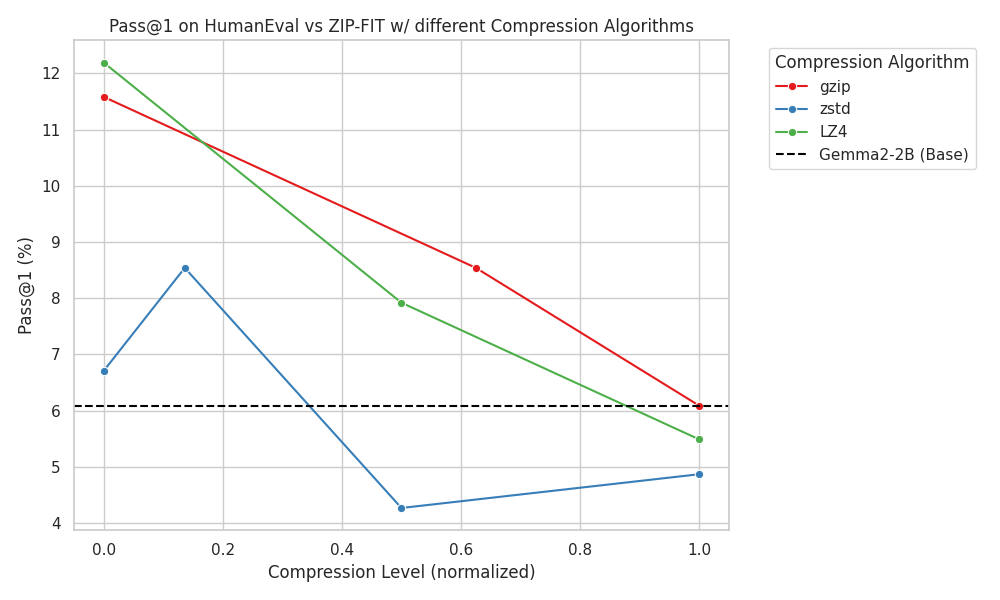
\includegraphics[width=\textwidth]{plots/zipf.png}
\caption{\textbf{Lighter compression preserves crucial information for data selection.} At minimum compression levels, both gzip and LZ4 achieve the strongest Pass@1 scores (11.58\% and 12.19\%), significantly outperforming the base model (6.09\%, dashed line). Performance systematically degrades with increased compression across all algorithms, suggesting that aggressive compression removes valuable alignment signals.}

\label{fig:compression_comparison}
\end{figure}

To investigate the impact of different compression algorithms on ZIP-FIT's performance, we conducted experiments comparing three widely used compression methods: gzip, zstd, and LZ4. Each algorithm was tested across its available compression levels, normalized to a 0-1 scale for comparison. As shown in Figure~\ref{fig:compression_comparison}, compression algorithm choice and level significantly impact performance.

Key findings include:
\begin{itemize}
    \item LZ4 at minimum compression achieves the best performance (12.19\% Pass@1)
    \item Higher compression levels generally lead to decreased performance across all algorithms
    \item gzip shows more stable performance degradation compared to LZ4 and zstd
    \item zstd consistently underperforms relative to both GZIP and LZ4
\end{itemize}

These results suggest that lighter compression better preserves the structural information needed for effective data selection. The superior performance of LZ4 at minimal compression indicates that aggressive data compression may remove subtle but important patterns useful for alignment assessment.

\newpage

\section{Data Selection Profiling (Run Times)}\label{sec:profiling_run_times}
\texttt{ZIP-FIT} performs selection up to 65.8\% faster than DSIR and 21,076\% (=5h/85s=211, which is 2 orders of magnitude) faster than D4. 
Experimental results comparing \texttt{ZIP-FIT} vs DSIR profiling/run time for Code data selection can be found in figure \ref{fig:profiling_run_times}. Note that depending on the dataset and number of samples these numbers may not hold. Compression may not scale well to long-context datasets and depending on the source dataset, our run times varied widely. However, on average we observed that \texttt{ZIP-FIT} is comparable to DSIR and generally faster. More experiments across a wider range of datasets need to be conducted in order to infer more.

\begin{figure*}[!ht]
    \centering
    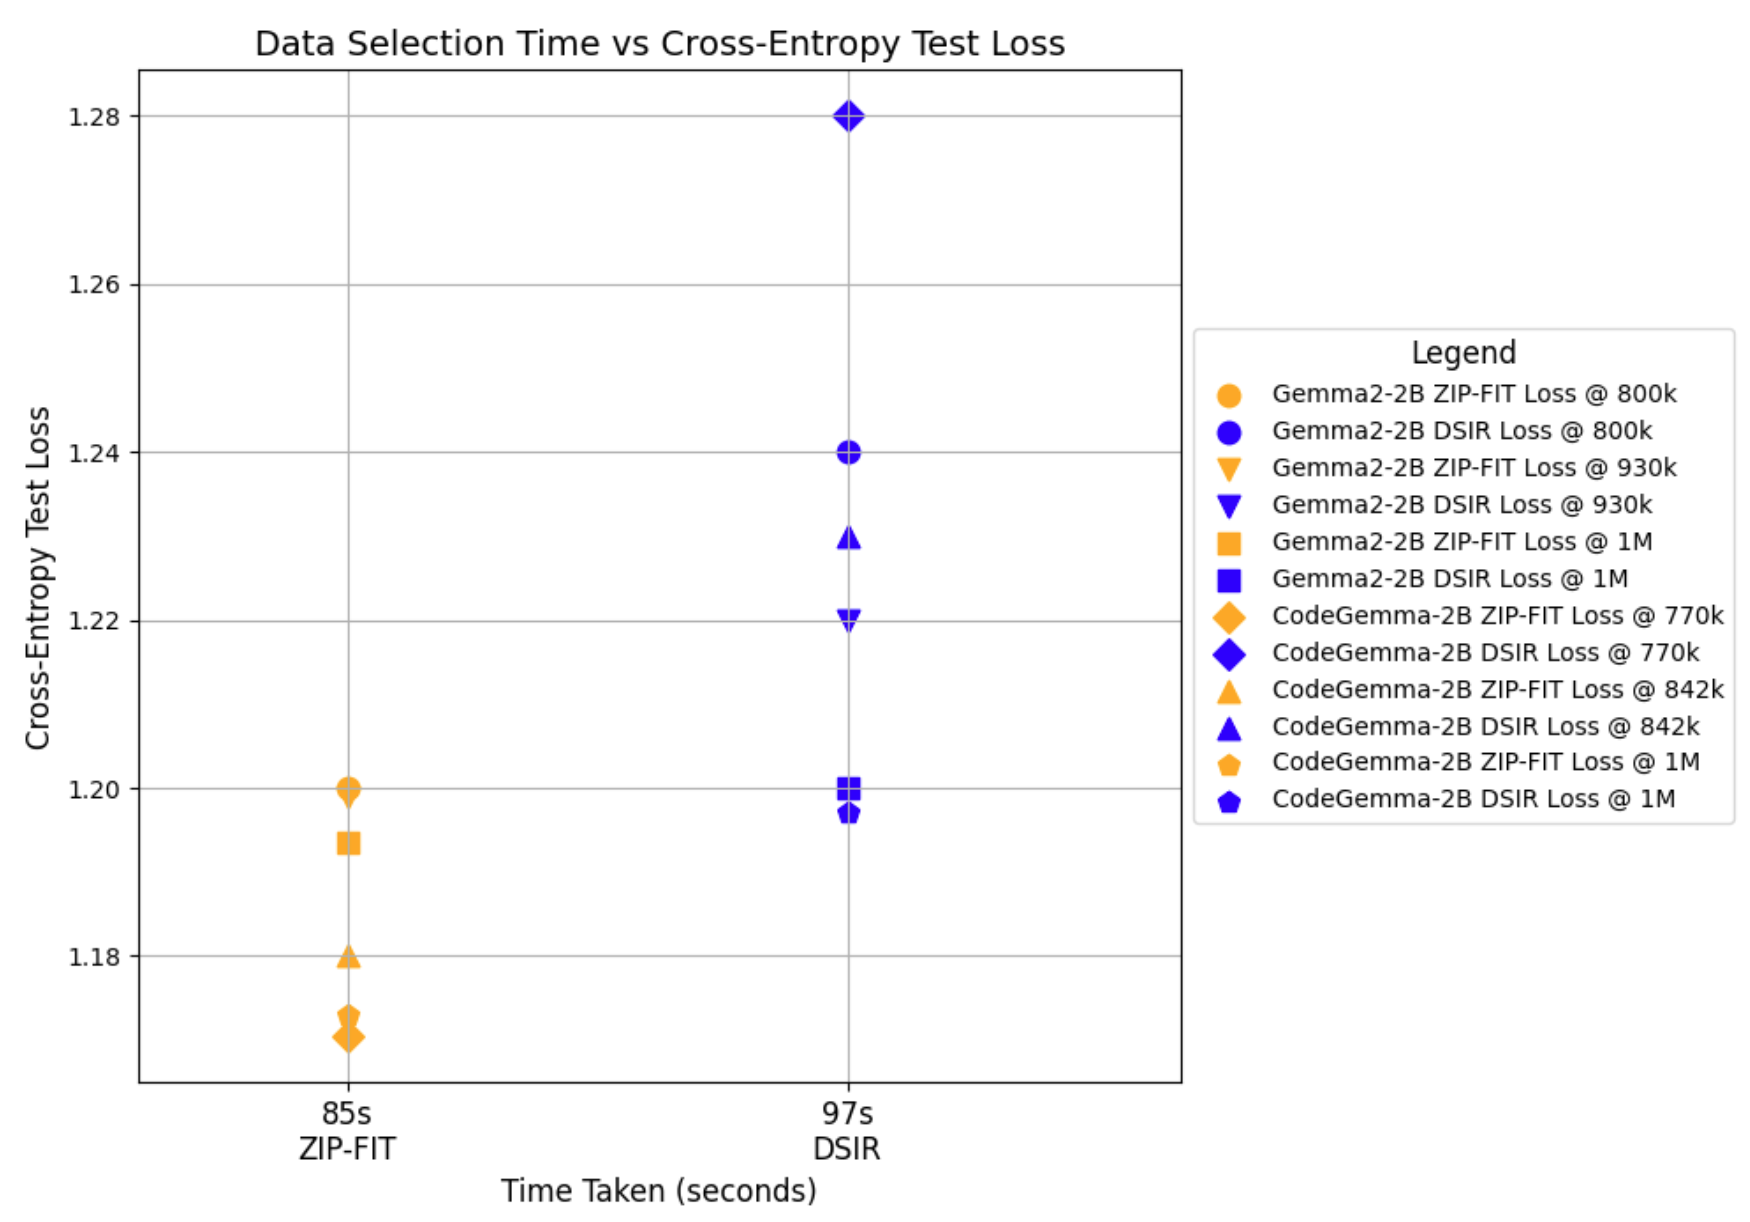
\includegraphics[width=0.8\textwidth]{plots/runtime_zip_fit_vs_dsir_code.png}
    \caption{\textbf{\texttt{ZIP-FIP} demonstrates lower cross-entropy and lower run time during data selection than competing DSIR and D4 methods.} 
    \texttt{ZIP-FIT} is cheaper, faster, and better performing. 
    The run times do no include fine-tuning time, since it’s a constant offset across all models. 
    D4's data selection (not shown) takes 5hs because it uses an embedding model (opt-125m \cite{opt}), the same one as the original paper \cite{d4}.
    }
    \label{fig:profiling_run_times}
\end{figure*}

\newpage

% % https://chatgpt.com/c/6704a8ae-51a4-8001-9930-39af597cc070
% \section*{Intuitive Explanation of Normalized Compression Distance (NCD): How Compression Measures Data Similarity}

% At the core of our methodology is a way to measure similarity between data points using compression. 
% Therefore, in this section, we conceptually explain how compression achieves this.  

% If \(x \sim x'\), meaning \(x\) and \(x'\) are similar, we expect the compressed size of their combination to be close to the compressed size of their shared core information, plus a small difference (delta). That is,

% \[
% C(x \oplus x') \sim C(x) + \text{delta}
% \]

% where \(\text{delta}\) represents the unique information added by \(x'\). To isolate this delta, we subtract the core shared information, represented by \(\min(C(x), C(x'))\), from the compressed size of the combination:

% \[
% C(x \oplus x') - \min(C(x), C(x'))
% \]

% This operation returns the delta, i.e., the additional information one object contributes beyond the shared core. Finally, normalization by \(\max(C(x), C(x'))\) scales this delta, keeping the distance bounded between 0 and 1.

% Dividing by the maximum, \( \max(C(x), C(x')) \), ensures that the Normalized Compression Distance (NCD) behaves as expected, remaining bounded between 0 and 1. When \( x \) and \( x' \) are very different, the compressed size of their combination is approximately the sum of their individual compressed sizes:

% \[
% C(x \oplus x') \approx C(x) + C(x')
% \]

% Substituting this into the NCD formula:

% \[
% \text{NCD}(x, x') = \frac{(C(x) + C(x')) - \min(C(x), C(x'))}{\max(C(x), C(x'))}
% \]

% we simplify the numerator to:

% \[
% (C(x) + C(x')) - \min(C(x), C(x')) = \max(C(x), C(x'))
% \]

% Thus, the NCD simplifies to:

% \[
% \text{NCD}(x, x') = \frac{\max(C(x), C(x'))}{\max(C(x), C(x'))} = 1
% \]

% This means that when \( x \) and \( x' \) are very different, the NCD approaches 1, indicating maximal dissimilarity. Dividing by the maximum also ensures that the NCD is normalized relative to the more complex object, properly scaling the distance. This avoids cases where differences would be exaggerated or diminished and guarantees that the NCD remains within the desired range of 0 to 1.

% The maximum, \( \max(C(x), C(x')) \), is used to normalize the NCD because it scales the distance relative to the more complex object, ensuring the measure reflects the proportional difference between the objects. When two objects are very different, the combined compressed size is dominated by the larger object, and using the maximum prevents smaller objects from distorting the distance calculation. This guarantees that the NCD stays bounded between 0 and 1, where 0 represents identical objects and 1 represents maximum dissimilarity. Dividing by the maximum also ensures that the measure remains intuitive across objects with varying complexities.

\section{Qualitative Analysis}
Qualitative results show top 20 examples can be found it table \ref{tab:code_top_20_zip_fit}.

\begin{table}[htbp]
    \centering
    \textbf{Selected Samples by \texttt{ZIP-FIT} with \texttt{ZIP-FIT} Alignment scores}\\[0.5em] 
    \begin{tabular}{|p{10cm}|c|}
        \hline
        \textbf{Sample Text (Beginning)} & \textbf{Alignment Score} \\ \hline
        Across all his bands and projects, Townsend has released twenty @-@ three studio albums and three live albums. & 0.5000 \\ \hline
        Require Import CodeDeps. Require Import Ident. Local Open Scope Z\_scope. Definition \_addr := 1\%positive. Definition \_g := 2\%positive. & 0.4928 \\ \hline
        This Photostock Vector Night Sky Background With Full Moon Clouds And Stars Vector Ilgraphicration has 1560 x 1560 pixel resolution... & 0.4926 \\ \hline
        module Structure.Logic where ... & 0.4926 \\ \hline
        \{ dg-do compile \} PR fortran/51993 Code contributed by Sebastien Bardeau \texttt{<bardeau at iram dot fr>} module mymod type :: mytyp... & 0.4891 \\ \hline
        For over ten years, the St. Louis Mercy home has formed a special connection with a local community theatre: The Muny. This summer the... & 0.4889 \\ \hline
        Read("SchreierSims.gi"); LoadPackage("AtlasRep"); MicroSeconds := function() local t; t := IO\_gettimeofday(); return t.tv\_sec * 1000000 + t.t & 0.4889 \\ \hline
        Get the keyId used by this peer (this peer's identifier). This is stored in the key store. & 0.4857 \\ \hline
        Initializes and adds a node to the graph. NOTE: At least the type must be supplied for the Node to exist in the graph. Args: graph: The graph... & 0.4853 \\ \hline
        def bgra2rgb(img): cv2.cvtColor(img, cv2.COLOR\_BGRA2BGR) has an issue removing the alpha channel, this gets rid of wrong trans... & 0.4853 \\ \hline
        % \texttt{\{\# LANGUAGE Strict, StrictData \#\} \{\# LANGUAGE DeriveGeneric, DeriveAnyClass \#\} \{\# LANGUAGE TypeFamilies, TypeFamilyDependencies \#\}...} & 0.4853 \\ \hline
        % \#include \texttt{<gsl/gsl\_math.h>} \#include "gsl\_cblas.h" \#include "cblas.h" void cblas\_drotmg (double *d1, double *d2, double *b1... & 0.4818 \\ \hline
        % Minnesota Starvation Experiment: To study the effects of diet and nutrition, Dr. Ancel Keys of the University of Minnesota Laboratory of Physiologi... & 0.4815 \\ \hline
        % \#include \texttt{<empool/ThreadPoolManager.h>} \#include \texttt{<empool/Mutex.h>} \#include \texttt{<empool/TaskBase.h>} \#include \texttt{<atomic>}... & 0.4815 \\ \hline
        % It’s in the details of 100,000 moments. What made you happy in the past 24 hours? Researchers asked 10,000 people this question... & 0.4779 \\ \hline
        % def run(*args: Any, **kwargs: Any) -> None: 'Run cwltool.' windows\_check() signal.signal(signal.SIGTERM, \_signal\_handler) try: & 0.4714 \\ \hline
        % Args: backbone: either a backbone module or a mmdet config dict that defines a backbone. The backbone takes a 4D image tensor and returns... & 0.4706 \\ \hline
        % \{ SPDX-License-Identifier: MIT \} \#include \texttt{<armnn/Descriptors.hpp>} \#include \texttt{<armnn/IRuntime.hpp>}... & 0.4706 \\ \hline
        % \{\# OPTIONS --no-positivity-check \#\} module STLC.Coquand.Completeness where open import STLC.Coquand.Normalisation public... & 0.4672 \\ \hline
        % // Copyright \texttt{©} 2017 Arm Ltd. All rights reserved. SPDX-License-Identifier: MIT & 0.4667 \\ \hline
    \end{tabular}\label{tab:code_top_20_zip_fit}
    \caption{Beginning characters of the top 20 samples selected by \texttt{ZIP-FIT} when the target task is code generation.}
\end{table}

\begin{table}[htbp]
    \centering
    \textbf{Selected Samples by DSIR with \texttt{ZIP-FIT} Alignment scores}\\[0.5em] 
    \begin{tabular}{|p{10cm}|c|}
        \hline
        \textbf{Sample Text (Beginning)} & \textbf{\texttt{ZIP-FIT} Alignment Score} \\ \hline
        \textless a href=``https://colab.research.google.com/github/julianovale/simulaca
        o\_python/blob/master/0006\_ex\_trem\_kronecker\_algebra\_computacao ... & 0.122 \\ 
        \hline
        library(qcc) \textbackslash\textbackslash n
        death=c(2,1,2,4,2,5,3,3,5,6,3,8,3,3,6,3,6,5,3,5,2,6,2,3,4,
        3,2,9,2,2,3,2,10,7,9,6,2,1,2,4,2,5,3,3,5,6,3,8,3,3,6,3,6,5,3,5,2,6,2 ... & 0.121 \\ 
        \hline
        gap \textgreater List(SymmetricGroup(4), p - \textgreater Permuted([1 .. 4], p)); \textbackslash\textbackslash n perms(4);
        [ [ 1, 2, 3, 4 ], [ 4, 2, 3, 1 ], [ 2, 4, 3, 1 ], [ 3, 2, 4, 1 ... & 0.191 \\
        \hline
        \# Solutions \textbackslash\textbackslash n
        \#\# Question 1 \textbackslash\textbackslash n
        \textgreater `1'. Using a `for' loop print the types of the variables in each of the
        \textgreater following iterables: \textbackslash\textbackslash n
        \textgreater  `1' ... & 0.145 \\
        \hline
        \# Some small pregroups \textbackslash\textbackslash n \# The lists of small pregroups were generated by \textbackslash\textbackslash n
        \# Chris Jefferson <caj21@st-andrews.ac.uk> and \textbackslash\textbackslash n ... & 0.195 \\ 
        \hline
        adjacency\_mat = [
        false true true true true true true true true false true true true true false 
        false false true false true false true false ... & 0.182 \\
        \hline
        \textbackslash section\{Lookup table used for accessing child voxels using a parent's 
        child descriptor\}
        \textbackslash label\{app:lookup-table\}
        \textbackslash lstset\{language=C,cap ... & 0.199 \\
        \hline
        \textbackslash* statistics \ test\_nist.c \textbackslash\textbackslash n * \textbackslash\textbackslash n * Copyright (C) 1996, 1997, 1998, 1999, 2000, 2007 Jim Davies, Brian Gough         \textbackslash\textbackslash n *         \textbackslash\textbackslash n * This pro ... & 0.180 \\
        \hline
        Problem Description Write a python function to find the first missing positive number. \textbackslash\textbackslash n def first\_Missing\_Positive(arr,n): \textbackslash\textbackslash n ptr = 0 ... & 0.239 \\
        \hline 
        import numpy as np \textbackslash\textbackslash n mandelTable = [[0,0,0,0,0,0,0,0,0,0,0,0,0,0,0,0,0,0,0,0,0,0,0,0,0,0,0,0,0,0,0,0,0, ... & 0.189 \\
        \hline
    \end{tabular}\label{tab:code_top_20_dsir}
    \caption{Beginning characters of the top 20 samples selected by DSIR when the target task is code generation. 
    DSIR does not easily provide alignment scores, so instead we report the \texttt{ZIP-FIT} scores, which reveals that \texttt{ZIP-FIT} doesn't score highly the DSIR examples which might explain why \texttt{ZIP-FIT} achieves better CE loss. 
    }
\end{table}

\section{Future Work (Cont.)}

\textbf{Lossless Compression for Alignment:} While \texttt{ZIP-FIT} has demonstrated substantial efficiency for data selection, there are several promising directions for future exploration. 
One potential enhancement is leveraging faster compression algorithms, such as \texttt{LZ4} and \texttt{Snappy}, which offer rapid processing speeds at the cost of lossy compression. 
In our current approach, we utilize \texttt{gzip} for compression-based alignment, which is lossless and provides a robust foundation. 
However, \texttt{LZ4} and \texttt{Snappy} are optimized for speed and could potentially offer even greater computational efficiency without the need for decompression in our pipeline. 
Given that our primary goal is efficient data selection rather than perfect data recovery, these faster algorithms might be more suitable. 

\textbf{Autonomous Validation Set Generation}: 
A current limitation of ZIP-FIT is its dependence on a small, curated validation set (e.g., 185 samples for ProofNet and 82 samples for half the HumanEval test set). 
Future work could explore the use of generative models to create synthetic validation sets from task-specific instructions. 
This approach could also be expanded to enable autonomous self-directed, model-driven generation of validation data. 






